\documentclass[colorlinks=true,linkcolor=blue]{beamer}
\usepackage{animate}
\usepackage{graphicx}

\usepackage{pdfpages}
\usepackage{hyperref}
\usepackage{array}
\newtheorem{remark}{Remark}
% \newtheorem{problem}{Problem}
\newtheorem{proposition}{Proposition}
\begin{document}
\begin{frame}
  \begin{center}

    {\Large Clustering}
    \end{center}
  \vskip 1in
{\small
Jeremy Teitelbaum \\
November 7, 2018 \\
UConn Math Club
}
\end{frame}
\begin{frame}
  \frametitle{Clustering: The basic problem}
\begin{center}
  \only<1>{
    \begin{block}{Results of an experiment:}
      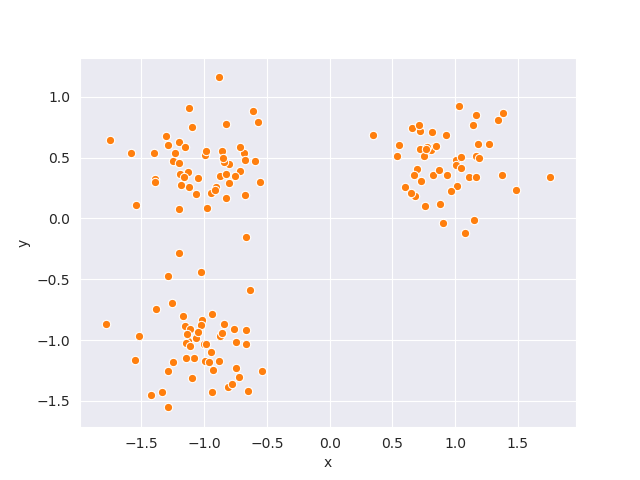
\includegraphics[width=3in]{../png/basic.png}
    \end{block}
  }
  \only<2>{\begin{block}{Looks like three things of interest:}
      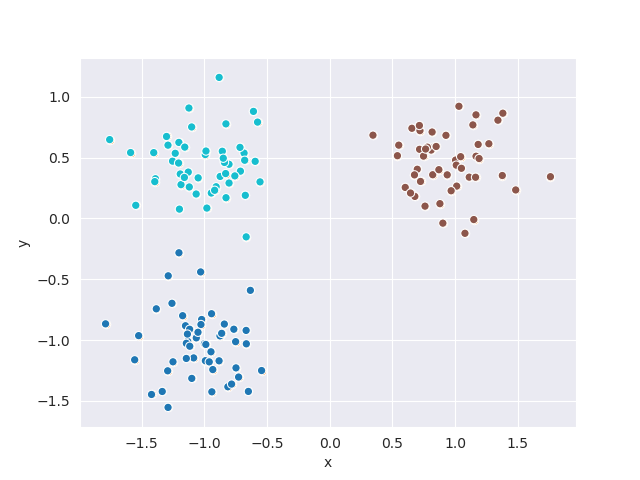
\includegraphics[width=3in]{../png/basic_1.png}
    \end{block}}
\end{center}
\end{frame}
\begin{frame}
  \begin{block}{How to pick them out?}
          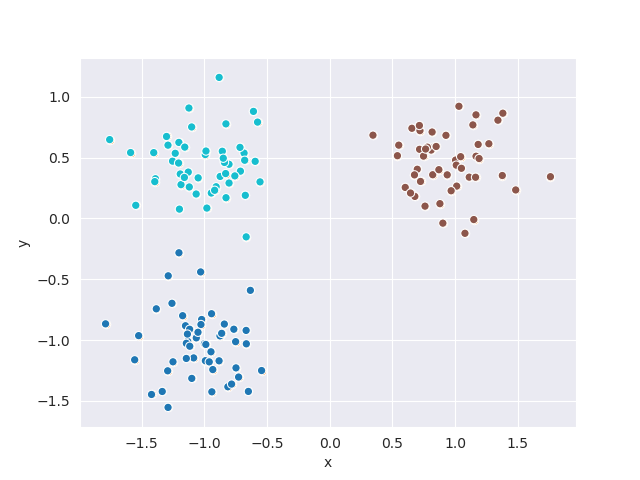
\includegraphics[width=3in]{../png/basic_1.png}
\end{block}
\end{frame}
\begin{frame}
  \begin{block}{Not so easy in high dimensions}<1->
\begin{center}
    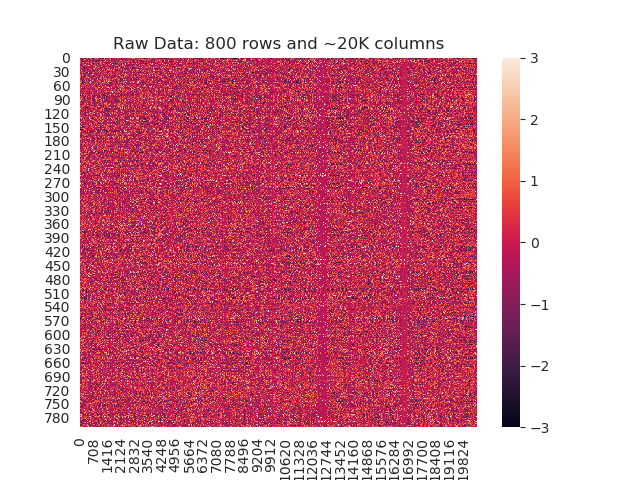
\includegraphics[width=3in]{../png/basic_image.png}
\end{center}
\end{block}
\begin{block}{Is there structure here?}<2>
  \end{block}
\end{frame}
\begin{frame}{Clustering}
  \begin{itemize}
  \item <1-> Clustering is a problem in {\it unsupervised machine learning}.
  \item <2-> Strategy 1: work from the bottom up.
  \item <3-> Strategy 2: work from the top down.
  \end{itemize}
\end{frame}
\begin{frame}{Bottom-Up (Hierarchical/Agglomerative) Clustering}

  \begin{block}{General Strategy}
    \begin{itemize}
    \item <1-> Group a few points that are very close together into clusters.
    \item<2-> Find the point not yet in a cluster, but closest to one of the existing clusters,
      and  add it to that closest cluster.
    \item<3-> Repeat step 2 until every point is in a cluster.
    \end{itemize}
  \end{block}
  \begin{block}{The Catch}<4->
    What is the distance between a point and a cluster?
    \end{block}
\end{frame}
\begin{frame}
  \frametitle{What is the distance to a cluster?}
  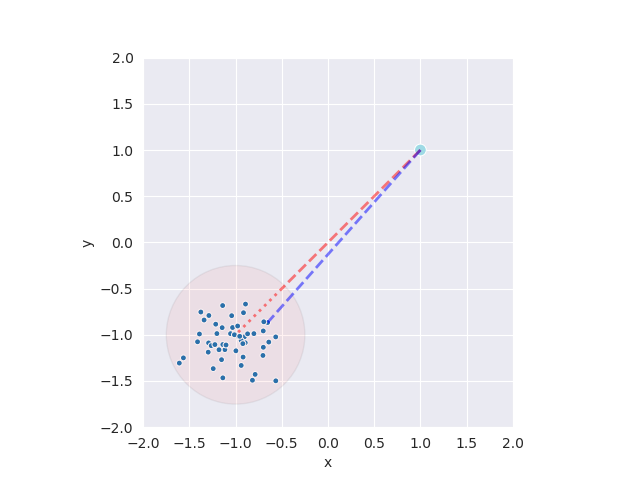
\includegraphics[width=4in]{../png/cluster_distance.png}
\end{frame}
\begin{frame}
  \frametitle{Different Notions of Distance}
  \begin{itemize}
  \item<1-> Distance between closest points.
    $$
    d(X,Y)=\inf_{(x,y)\in X\times Y} d(x,y)
    $$
    
  \item<2-> Distance between farthest points.
    $$
    d(X,Y)=\max_{(x,y)\in X\times Y} d(x,y)
    $$
  \item<3-> Distance between centroids.
    $$
    d(X,Y)=d(\overline{X},\overline{Y})
    $$
  \end{itemize}
\end{frame}
\begin{frame}
  \frametitle{Some Test Cases}
  \begin{center}
    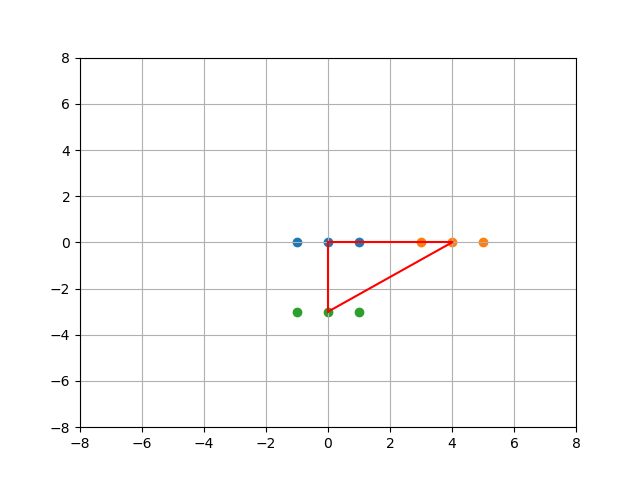
\includegraphics[width=4in]{../png/centroid.png}
  \end{center}
\end{frame}
\begin{frame}
  \frametitle{Algorithmic Considerations}
  \begin{definition} Let $X_i$ be a set of $k$ clusters.  The ``dissimilarity matrix'' is the symmetric $k\times k$
    matrix whose $(i,j)$-entry is $d(X_i,X_j)$.
  \end{definition}
\begin{block}{Algorithm}
  \begin{enumerate}
  \item Given $n$ points $y_i$ to start, construct  the $n\times n$ symmetric matrix $D_0$ whose entries
    are the $d(y_i,y_j)$.  Set $N=0$.
  \item Find the two closest points (later clusters) by finding $i',j'$ where $D_N(i',j')$ is minimal.
  \item Combine the two points into a cluster $c_0$.  Update $D_N$ by removing the two points $y_{i'}$ and $y_{j'}$ and
    adding a row and column for the distances between the remaining points and $c_0$, yielding $D_{N+1}$.
  \item Repeat steps $2$ and $3$ until you have only one cluster.
  \end{enumerate}
\end{block}
\end{frame}
\begin{frame}
  \frametitle{Algorithmic Considerations (cont'd)}
  To make this approach efficient, we want to be able to update the dissimilarity matrix without recomputing all of the distances from scratch.

  When the distance between clusters is the distance between their closest points, or the distance between their farthest points, this is straightforward.

  \begin{itemize}
  \item (closest): If $X$ and $Y$ are merged, and $Z$ is another cluster, then the distance $d(Z,X\cup Y)$ is
    $\min(d(X,Z),d(Y,Z))$ and this can be computed directly from the dissimilarity matrix $D$.
    \item (farthest): If $X$ and $Y$ are merged, and $Z$ is another cluster, then the distance $d(Z,X\cup Y)$ is
    $\max(d(X,Z),d(Y,Z))$ and this can be computed directly from the dissimilarity matrix $D$.
    \item What about centroids?
  \end{itemize}
\end{frame}
\begin{frame}
  \frametitle{A geometry problem}
  \begin{problem}<1->
   Let $X=\{x_1,\ldots, x_{n_x}\}$, $Y=\{y_1,\ldots,y_{n_y}\}$ and $Z=\{z_1, \ldots, z_{n_z}\}$ be three sets
    of points in
    $\mathbf{R}^{m}$ and let $\overline{x}$, $\overline{y}$, and $\overline{z}$ be their respective centroids.
    Find the centroid of the merged set $X\cup Y$
    and the distances between that centroid and $\overline{z}$ as efficiently as you can.
  \end{problem}
\begin{block}{}<2->
  Recall that the centroid of a set of points is their (vector) average:
  $$
  \overline{x}=\frac{1}{n_x}\sum_{i=1}^{n_x} x.
  $$

  Let $A=X\cup Y$ and $\overline{a}$ be the centroid of $A$.
  The centroid of the merged set could be computed from the original points, but a more efficient approach
  is to observe that
  $$
  \overline{a}=\frac{n_x\overline{x}+n_y\overline{y}}{n_x+n_y}
  $$
\end{block}
\end{frame}
\begin{frame}
 Since knowing the sizes of the clusters is going to be helpful, lets assume we keep track not only of the dissimilarity matrix $D$ but also the sizes $n_X$ for each cluster $X$.  Initially, all $n_X=1$.

The remaining piece of our geometry problem is:
\begin{problem} Write $d(\overline{a},\overline{z})=|\overline{a}-\overline{z}|$ in terms of $n_x, n_y, n_z$ and $\overline{x}$, $\overline{y}$, and $\overline{z}$.
\end{problem}

\begin{proposition} We have
  $$
  |\overline{a}-\overline{z}|^2 =\frac{n_x}{n_x+n_y}|\overline{x}-\overline{z}|^2+\frac{n_y}{n_x+n_y}|\overline{y}-\overline{z}|^2-\frac{n_x n_y}{(n_x+n_y)^2}|\overline{x}-\overline{y}|^2
  $$
  \end{proposition}

  \begin{remark} It's much easier to work directly with the squared Euclidean distance than the usual one when making and updating the dissimilarity matrix.
    \end{remark}
  
\end{frame}
\begin{frame}
  \frametitle{Ward's Criterion}
  Ward's criterion is an additional way to decide which clusters are closest and should be merged next.

  \begin{definition} If $X$ is a cluster, the 'within cluster' sum-of-squared error is
    $$
    s(X)=\sum_{i=1}^{n_x} (x-\overline{x})^2
    $$
    The error $S$ is the sum of this over all clusters:
    $$S=\sum_{X} s(X).$$
  \end{definition}

  Notice that at the beginning of the clustering process, when all the clusters have only one point, $S=0$.
  Ward's criterion says that \textit{when merging clusters, always choose the two that increase $S$ by
    the least amount.}
\end{frame}
\begin{frame}
  \frametitle{Ward's Criterion (cont'd)}
  \begin{proposition} When two clusters with sizes $n_x$ and $n_y$, and centroids $\overline{x}$ and $\overline{y}$, are merged, the increase in $S$ is given by
    $$
    \Delta S=\frac{n_x n_y}{(n_x+n_y)} (|\overline{x}-\overline{y}|^2)
    $$
  \end{proposition}

  So one way to look at Ward's method is that it combines the closest clusters by their centroid distances, but it weights those distances by the sizes of the clusters.  It prefers to merge smaller clusters.
  
\end{frame}
\begin{frame}
\begin{center}
  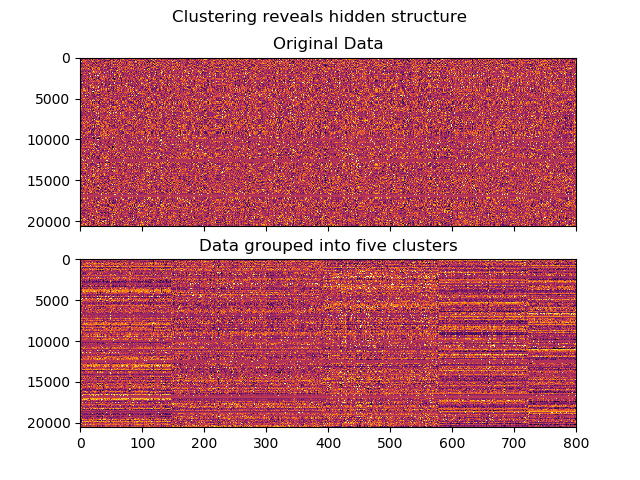
\includegraphics[width=4.5in]{../png/reveal.png}
\end{center}
\end{frame}
\begin{frame}
  \frametitle{Principal Component Analysis}
\begin{center}
  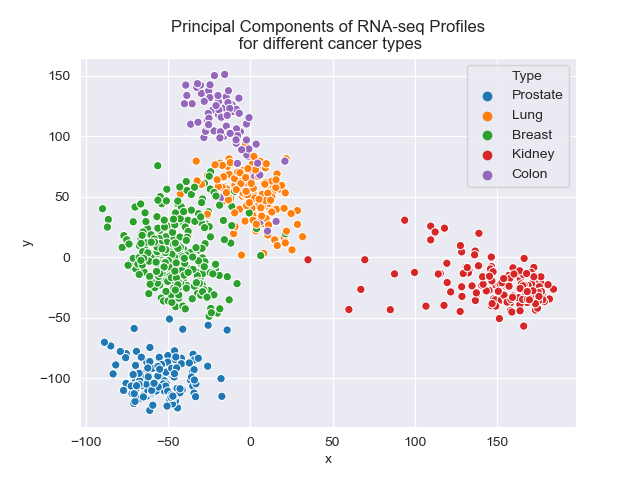
\includegraphics[width=3in]{../png/cluster.png}
\end{center}
This slide is for those who saw the PCA talk a few weeks ago.  
\end{frame}
\begin{frame}
  \frametitle{Top Down Clustering}
  Hierarchical or Agglomerative Clustering works from the bottom up. The most common top-down algorithm is called ``k-means clustering.''
  \begin{enumerate}
  \item Decide in advance how many clusters (say, $k$) that you want to find. (How? good question!)
  \item Pick $k$ points at random in the space of data. Call these points $m_1, \ldots, m_k$. 
  \item For each data point, find the closest of the $m_i$ and put your point in that ``cluster.''
  \item For each ``cluster'', compute the centroid, yielding new means $m_1', \ldots, m_k'$.
  \item Repeat until the $m_i$ stop moving.
  \end{enumerate}
\end{frame}
\begin{frame}
\begin{center}
    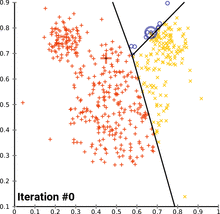
\includegraphics[width=1in]{../png/kmeans/kmeans-0.png}<1>%
    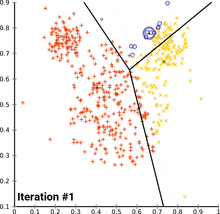
\includegraphics[width=1in]{../png/kmeans/kmeans-1.png}<2>%
    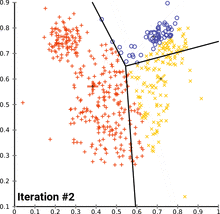
\includegraphics[width=1in]{../png/kmeans/kmeans-2.png}<3>%
    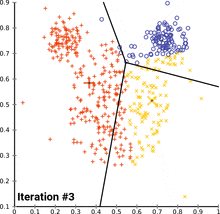
\includegraphics[width=1in]{../png/kmeans/kmeans-3.png}<4>%
    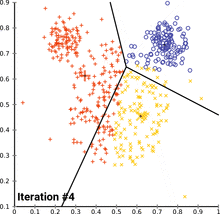
\includegraphics[width=1in]{../png/kmeans/kmeans-4.png}<5>%
    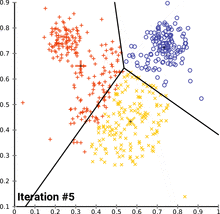
\includegraphics[width=1in]{../png/kmeans/kmeans-5.png}<6>%
    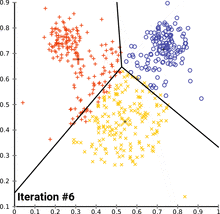
\includegraphics[width=1in]{../png/kmeans/kmeans-6.png}<7>%
    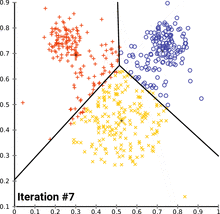
\includegraphics[width=1in]{../png/kmeans/kmeans-7.png}<8>%
    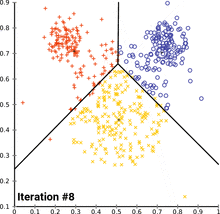
\includegraphics[width=1in]{../png/kmeans/kmeans-8.png}<9>%
    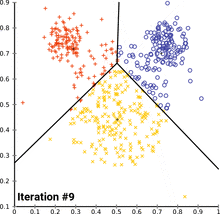
\includegraphics[width=1in]{../png/kmeans/kmeans-9.png}<10>%
   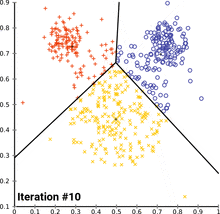
\includegraphics[width=1in]{../png/kmeans/kmeans-10.png}<11>%
   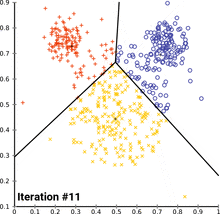
\includegraphics[width=1in]{../png/kmeans/kmeans-11.png}<12>%
    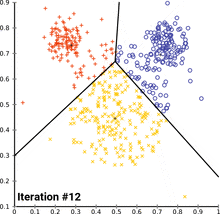
\includegraphics[width=1in]{../png/kmeans/kmeans-12.png}<13>%
    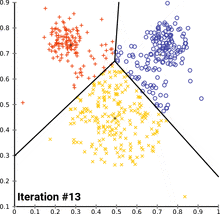
\includegraphics[width=1in]{../png/kmeans/kmeans-13.png}<14>%
    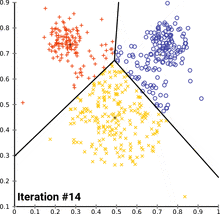
\includegraphics[width=1in]{../png/kmeans/kmeans-14.png}<15>%
  \end{center}
With thanks to \href{https://en.wikipedia.org/wiki/K-means_clustering}{Wikipedia}.
\end{frame}
\begin{frame}{Further Reading}
  For those interested in applying clustering algorithms, there is a powerful set of tools in the Python
  \texttt{scikit-learn} library and in  many \texttt{R} packages.
  \end{frame}
  \end{document}